\documentclass[usernames,dvipsnames]{beamer}

\usepackage[utf8]{inputenc}
\usepackage{epstopdf}
\usepackage{textpos}
\usepackage{textcomp}
\usepackage{verbatim}
\usepackage{varwidth}
\usepackage{amsmath}
\usepackage{amsfonts}
\usepackage{algorithmic}
\usepackage[linesnumbered,ruled]{algorithm2e}
\usepackage{graphicx}
\usepackage{xcolor}
\usepackage{listings}
%\usepackage{lipsum}
%\usepackage{dblfloatfix}
%\usepackage{multicol}
%\usepackage[ruled]{algorithm2e}

\lstset{%frame=tb,
language=C++,
aboveskip=3mm,
belowskip=3mm,
showstringspaces=false,
columns=flexible,
basicstyle={\small\ttfamily},
numbers=none,
numberstyle=\tiny\color{gray},
keywordstyle=\color{blue},
commentstyle=\color{OliveGreen},
%commentstyle=\color{green},
%commentstyle=\color{dkgreen},
stringstyle=\color{mauve},
breaklines=true,
breakatwhitespace=true,
tabsize=3
}

\usefonttheme[onlymath]{serif}
%\setlength{\columnsep}{5cm}

% table of contents font size
\setbeamerfont{section in toc}{size=\footnotesize}
\setbeamerfont{subsection in toc}{size=\scriptsize}
\setbeamerfont{subsubsection in toc}{size=\scriptsize}

\setbeamertemplate{caption}[numbered]

% standard, good-looking theme
\usetheme{Madrid}

% this should put the outline on the header of each page
% can't make it look right, though
% \usetheme{Darmstadt}



\title[Capstone]{Parallel Orthogonal Recursive Bisection (ORB)}

%\author{Team Metropolis:\\ James Farzi, JJ Lay, Graham West}
%\date{April 19, 2019}
\date{}

%\titlegraphic{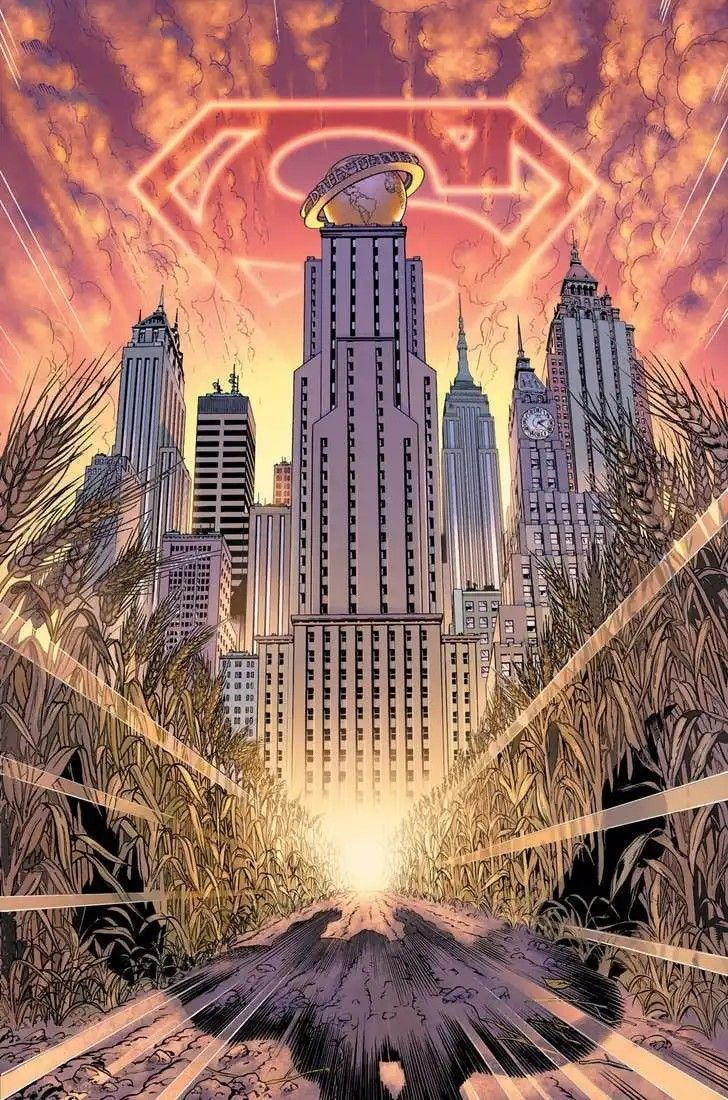
\includegraphics[width=0.9\textwidth]{images/DailyPlanet}}


%%%%%%%%% BEGIN DOCUMENT %%%%%%%%%
%%%%%%%%% BEGIN DOCUMENT %%%%%%%%%
%%%%%%%%% BEGIN DOCUMENT %%%%%%%%%

\begin{document}

% get title page 
\begin{frame}
	\titlepage
	
	\vspace{-65pt}
		
	\minipage{0.5\textwidth}
		\centering
		\textbf{Team Metropolis: \\
		\textcolor{red}{James Farzi}, \textcolor{Goldenrod}{JJ Lay}, \\ \textcolor{blue}{Graham West}} \\
		\vspace{7pt}
		April 19, 2019 \\
		\vspace{7pt}
		COMS 7900, Capstone \\
		\vspace{4pt}
		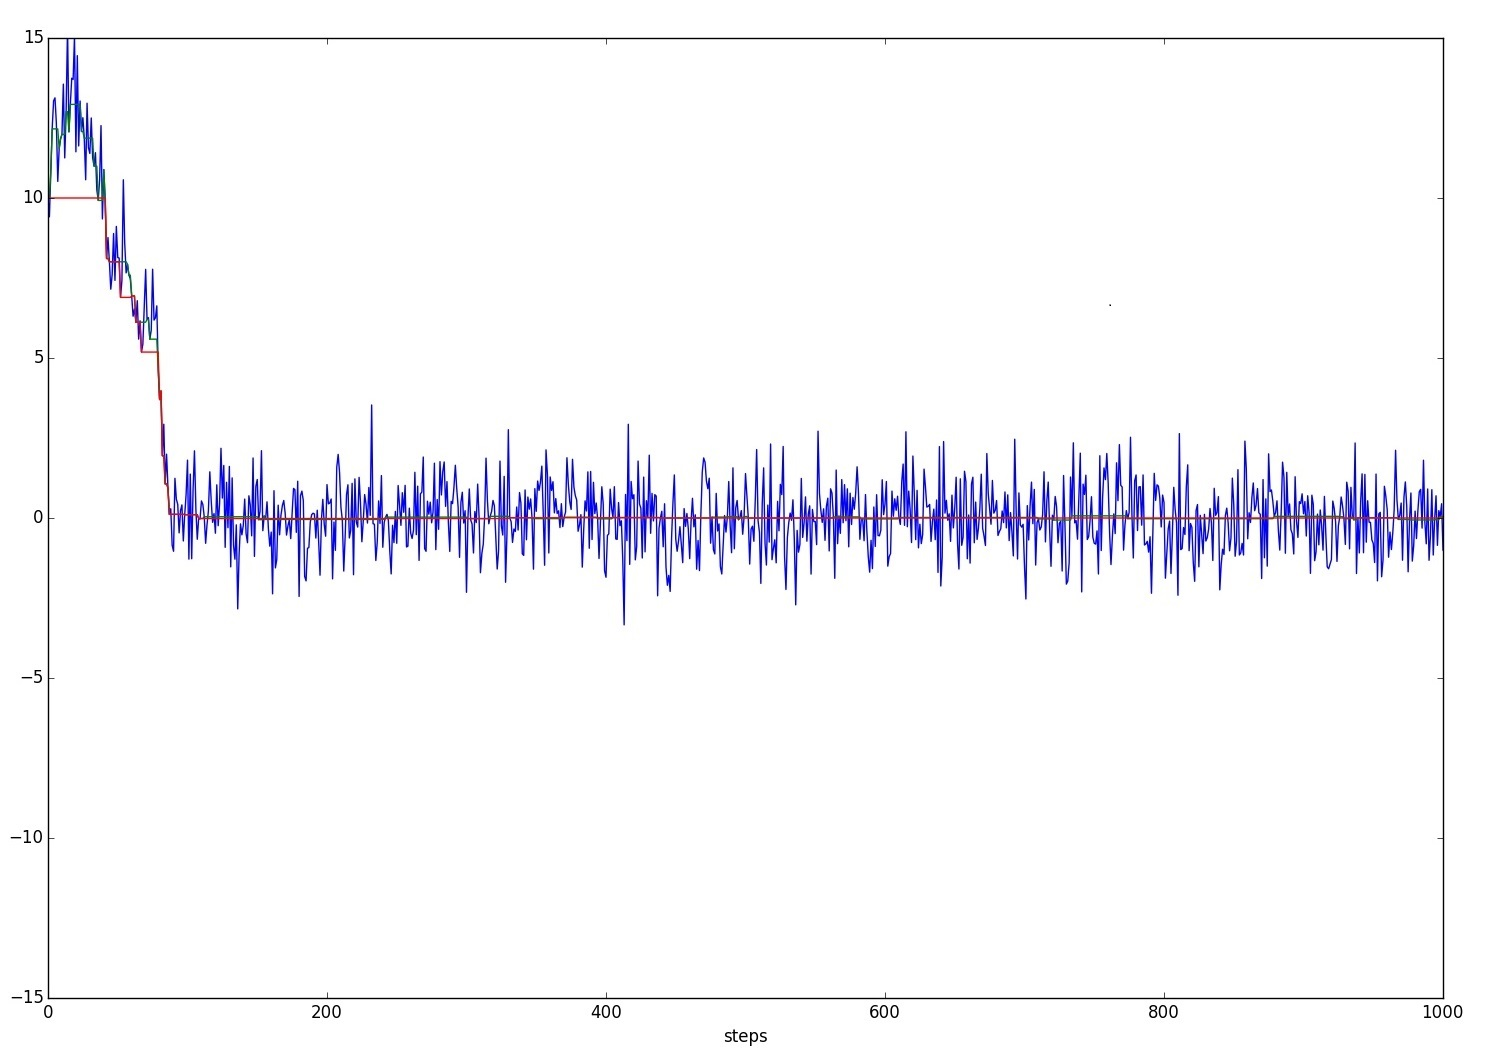
\includegraphics[scale = 0.17]{images/MCMC_Plot}
	\endminipage\hfill %%%%%%%%%%%%%%%%%%%
	\minipage{0.5\textwidth}
		\centering
		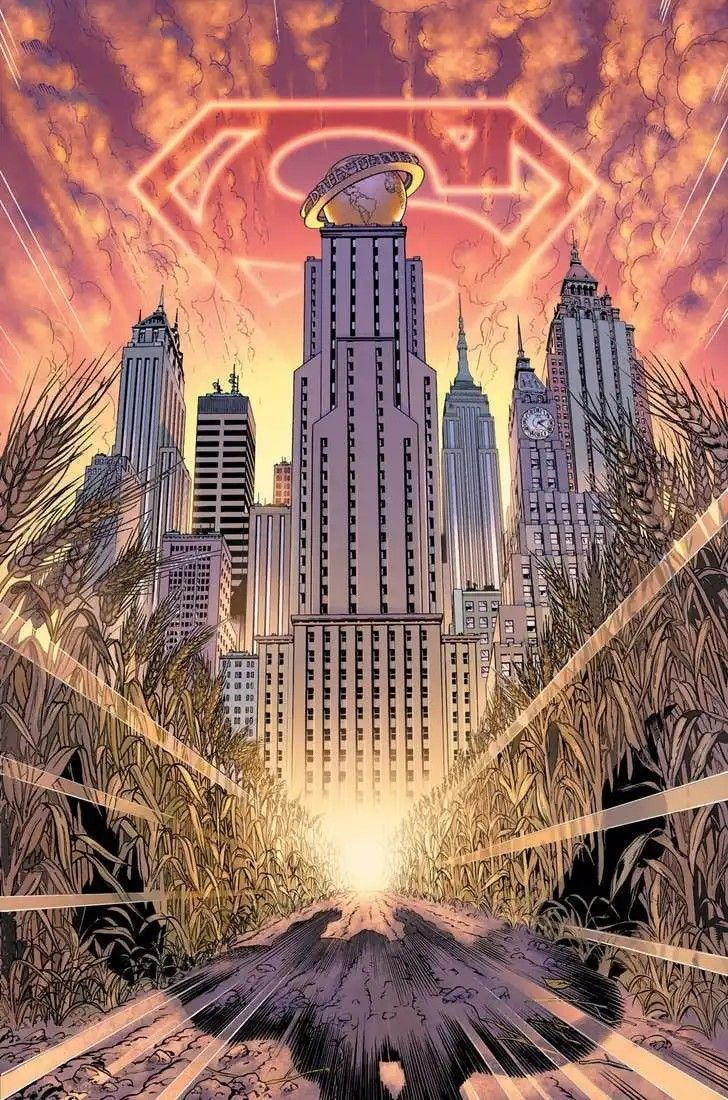
\includegraphics[scale = 0.17]{images/DailyPlanet}
	\endminipage\hfill
	
\end{frame}

\begin{frame}	
	\frametitle{Outline}
	\tableofcontents
\end{frame}


%%%%%%%%%%%%%
%%% NEW SECTION %%%
%%%%%%%%%%%%%
\section{Introduction}

\begin{frame}	
	\begin{Huge}
		\begin{center}
			Introduction
		\end{center}
	\end{Huge}
\end{frame}

\begin{frame}	
    \frametitle{Introduction}
    	
    	Expansion upon previous parallel sorting project
    	
    	\vspace{10pt}
    	
    	\begin{block}{Objectives:}
    		\begin{itemize}
    			\item Given a large set of data
    			\item Develop parallel orthogonal recursive bisection (ORB) algorithm
    			\item Utilize a $k$-d tree to organize data
    			\item Maximize use of MPI using multiple nodes
    			\item Requires both serial/parallel build/search operations
    			\item Search for nearest neighbors in the $k$-d data with a list of points and 3 radii
    		\end{itemize}
    	\end{block}
\end{frame}

\begin{frame}	
    \frametitle{Introduction}
    	\begin{block}{Workflow:}
    		\begin{itemize}
			\setlength\itemsep{0.5pt}
   			\item Prototyping: implementation based on Graham's MATLAB code
   			\item Extreme coding is FUN...and powerful
    			\item Used C++ w/ C MPI calls
    			\item Using Git effectively:
    				\begin{itemize}
					\setlength\itemsep{0.5pt}
    					\item Master and sub branches
    					\item Reduced merge conflicts
				\end{itemize}
    			\item Execution:
    				\begin{itemize}
					\setlength\itemsep{0.5pt}
    					\item \texttt{qlogin}
    					\item \texttt{qsub}
				\end{itemize}
    			\item Debugging:
    				\begin{itemize}
					\setlength\itemsep{0.5pt}
    					\item \texttt{valgrind}
    					\item \texttt{gdb}
				\end{itemize}
   			\item Output sorting:
    				\begin{itemize}
					\setlength\itemsep{0.5pt}
    					\item \texttt{sleep(myRank)}
    					\item Prepend a numeric key on \texttt{cout}'s
				\end{itemize}
    		\end{itemize}
    	\end{block}
\end{frame}




%%%%%%%%%%%%%
%%% NEW SECTION %%%
%%%%%%%%%%%%%
\section{Implementation}

\begin{frame}	
	\begin{Huge}
		\begin{center}
			Implementation
		\end{center}
	\end{Huge}
\end{frame}

\subsection{\texttt{main}}

\begin{frame}
	\frametitle{\texttt{main}}
	
	Our \texttt{main} was quite simple due to our organization of the project into many levels of functions
	
	\vspace{10pt}
	
	We also were able to use much of the basic initialization and data importing functions from the previous project
	
	\vspace{10pt}
	
	\begin{algorithm}[H]
%		\footnotesize
		\begin{algorithmic}[1]
			\STATE Initialize MPI
			\STATE Set number of files, lines per file to read
			\STATE import the $data$
%			\STATE MPI\_Barrier
			\STATE Initialize $tree$
			\STATE \texttt{buildTree}($data$, $tree$, $comm$, $\cdots$)
%			\STATE MPI\_Barrier
			\STATE Search the tree with \texttt{search501}( $tree$, $\cdots$)
%			\STATE MPI\_Barrier
			\STATE Finalize MPI
		\end{algorithmic}
	\caption{\texttt{main}($\cdots$)}
	\end{algorithm}
		
\end{frame}

%%%%%
%
% Subsection: Importing Data
%
%%%%%

\subsection{Importing Data}

%%%%
% Importing data
%%%%

\begin{frame}
	\frametitle{Importing Data}
	
    	\begin{block}{Importing the data:}
	    	
    		\texttt{listFiles}($\cdots$)
    		\begin{itemize}
    			\item Fetches a list of data filenames using OS calls (random order)
    		\end{itemize}
    		
    		\texttt{distributeFiles}($\cdots$), \texttt{receiveFiles}($\cdots$)
    		\begin{itemize}
    			\item Isend/Recv the list of filenames
    			\item Round robin distribution of files
    		\end{itemize}
    		
    		\texttt{importFiles}($\cdots$)
    		\begin{itemize}
    			\item Reads the received filenames
    			\item Read a set nFiles and nLinesPerFile
    			\item Returns a 1D array of length 4 $\times$ nFiles $\times$ nLinesPerFile
    			\item nFiles $\ge$ nNodes
    		\end{itemize}
    		
    		\texttt{CalculateIndex($\cdots$)}
    		    \begin{itemize}
    		        \item Calculates the starting index of the first row
    		    \end{itemize}
    	\end{block}
		
\end{frame}

%%%%
% listFiles
%%%%

\begin{frame}
	\frametitle{\texttt{listFiles}}
	
    		\texttt{vector<string> listFiles(string path, int numFiles )}
    		\begin{itemize}
    			\item Fetches a list of data filenames using \texttt{opendir} from \texttt{path}
    			\item Files are returned in ``random'' order
    			\item Returns list as a \texttt{vector} of \texttt{string}
    			\item Maximum number of files returned is \texttt{numFiles}
    		\end{itemize}
    		

\end{frame}

%%%%
% distributeFiles
%%%%

\begin{frame}
	\frametitle{\texttt{distributeFiles}}
	
    		\texttt{void distributeFiles(vector<string> files, int numWorkers)}
    		\begin{itemize}
    		    \item Asynchronously transmits filenames in \texttt{files} to nodes
    			\item Used \texttt{MPI\_Isend} since it sends to itself
    			\item Round robin distribution of files
    			\item Transmits the string ``DONE!'' to all nodes at end
    		\end{itemize}
    		
\end{frame}


%%%%
% receiveFiles
%%%%

\begin{frame}
	\frametitle{\texttt{receiveFiles}}
	
    		\texttt{vector<string> receiveFiles(int myRank)}
    		\begin{itemize}
    			\item Asychronously receives filenames from rank 0
    			\item Used \texttt{MPI\_Irecv} and \texttt{MPI\_Wait}
    		\end{itemize}
    		
\end{frame}


%%%%
% importFiles
%%%%

\begin{frame}
	\frametitle{\texttt{importFiles}}
	
	\begin{tabular}{l l}
    		\texttt{void importFiles(} & \texttt{vector<string> files, int myRank,} \\
	& \texttt{float *myData, int *rows, int *cols,} \\
	& \texttt{int maxRowsPerFile,} \\
	& \texttt{unsigned long int arrayLimit)} \\
	\end{tabular}
	
    		\begin{itemize}
    			\item Read a set nFiles and nLinesPerFile
    			\item Returns a 1D array of length 4 $\times$ nFiles $\times$ nLinesPerFile
    			\item nFiles $\ge$ nNodes
    		\end{itemize}
    		
\end{frame}


%%%%
% CalculateIndex
%%%%

\begin{frame}
	\frametitle{\texttt{CalculateIndex}}
	
    		\texttt{float CalculateIndex(string filename)}
    		    \begin{itemize}
    		        \item Calculates the starting index ($I_0$) of the first row of the given file
    		        \item If $x$ is the five digit integer in the filename and $R_{\max}$ is the maximum number of rows in a file, then \\ 
    		        $I_0 = (x - 1) * R_{\max}$
                    \item Returns a float to avoid using a separate data type for the index and allows using a single 1D array for the four fields
    		    \end{itemize}

\end{frame}

%%%%%
%
% Subsection: Tree Structure
%
%%%%%

\subsection{Tree Structure}

%%%%
% Old tree structure
%%%%

\begin{frame}[fragile]
	\frametitle{Tree Structure}
	
    	\begin{block}{Old tree struct:}
    		\begin{itemize}
    			\item Contained extra debugging fields
    			\item Contained completely unused fields
    			\item Originally used doubles
    			\item tree naming
    		\end{itemize}
    	\end{block}
\end{frame}

%%%%
% New tree structure
%%%%

\begin{frame}[fragile]
	\frametitle{Tree Structure}

\begin{block}{New tree struct:}
\lstset{
   basicstyle=\tiny
}
\begin{lstlisting}{language=C++}
struct Tree {
   Tree *p;  // Parent
   Tree *l;  // Left child
   Tree *r;  // Right child

   MPI_Comm parentComm, leftComm, rightComm, thisComm;

   float x1;  // Min x
   float x2;  // Max x
   float y1;  // Min y
   float y2;  // Max y
   float z1;  // Min z
   float z2;  // Max z

   float c[4];  // Center of this tree
   float radius;

   float d[4];  // Data point
}
\end{lstlisting}
\end{block}
\end{frame}

%%%%
% C Constants
%%%%

\begin{frame}
	\frametitle{C Constants}
	
    \begin{block}{\texttt{definitions.h}:}
        A header file containing numerous preprocessor identifiers (\texttt{\#define}) to improve code readability and reduce the number of constant values:
        \begin{itemize}
            \item Array indexing
                \begin{itemize}
                    \item \texttt{\#define \_X\_ 1} $\rightarrow$  \\
                    \texttt{var = data[\_X\_]}
                    \item \texttt{\#define mpi\_Max\_Filename 200} $\rightarrow$ \\
                    \texttt{auto name = new char[mpi\_Max\_Filename]}
                \end{itemize}
            \item MPI tags
                \begin{itemize}
                    \item \texttt{\#define mpi\_Tag\_File 30} $\rightarrow$ \\
                    \texttt{MPI\_Send(name, sz, MPI\_CHAR, Rank0, mpi\_Tag\_File, \ldots}
                \end{itemize}
            \item Count limits
                \begin{itemize}
                    \item \texttt{\#define abortCount 5000} $\rightarrow$ \\
                    \texttt{while (i < abortCount)}
                \end{itemize}
    		\end{itemize}
    	\end{block}
		
\end{frame}

\subsubsection{Building the tree}

\begin{frame}
	\frametitle{Building the tree}
	
	To build the tree, we use several functions which perform different aspects/sections of the task
	
	\vspace{10pt}
	
	\begin{block}{Functions:}
		\begin{itemize}
			\item \texttt{buildTree}
			\item \texttt{buildTree\_serial}
			\item \texttt{buildTree\_parallel}
			\item \texttt{getSortDim}
		\end{itemize}
	\end{block}
\end{frame}

%%%
% Building the tree
% Communicator diagram
%%%

\begin{frame}
	\frametitle{Building the tree}
	    \begin{figure}[h!]
       	    \centering
            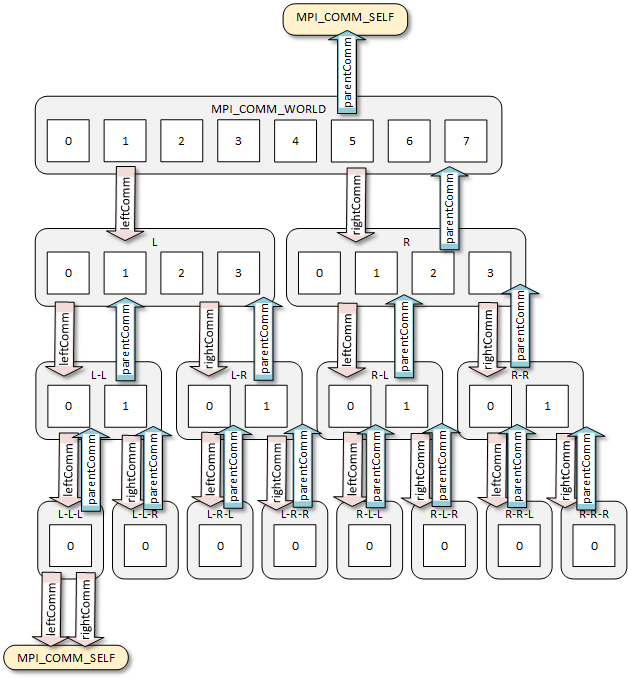
\includegraphics[width=0.5\textwidth]{images/communicators.png}
            \caption{Example of parallel variables using eight nodes}
            \label{fig:communicators}
        \end{figure}
\end{frame}

\begin{frame}
	\frametitle{Building the tree}
	
	\texttt{buildTree} checks the number of compute nodes in the current communicator and determines whether to call the parallel or serial versions of the code
	
	\vspace{10pt}
	
	\begin{algorithm}[H]
		\begin{algorithmic}[1]
			\STATE $q$ = Size of current communicator
			\IF{ $q > 1$}
				\STATE \texttt{buildTree\_parallel}($data$, $tree$, $comm, \cdots$)
			\ELSE
				\STATE \texttt{buildTree\_serial}($data$, $tree$, $\cdots$)
			\ENDIF
		\end{algorithmic}
	\caption{\texttt{buildTree}($data$, $tree$, $comm, \cdots$)}
	\end{algorithm}
		
\end{frame}

\begin{frame}
	\frametitle{Building the tree}
	
	\texttt{buildTree\_parallel} performs ORB using multiple compute nodes
	
	\vspace{10pt}
	
	\begin{algorithm}[H]
		\footnotesize
		\begin{algorithmic}[1]
			\STATE Call \texttt{getSortDim}($\cdots$): calculates $x,y,z$ mins, maxs, ranges, partition center, and returns $sortDim$
			\STATE Sort $data$ over $sortDim$ using \texttt{parallelSort}($data$, $sortDim$, $comm$, $\cdots$ )
			\IF{ $myRank < numNodes/2$ }
				\STATE Create $tree.L$, $commL$
				\STATE \texttt{buildTree\_parallel}( $data$, $tree.L$, $comm, \cdots$ )
			\ELSE
				\STATE Create $tree.R$, $commR$
				\STATE \texttt{buildTree\_parallel}( $data$, $tree.R$, $comm, \cdots$ )
			\ENDIF
		\end{algorithmic}
		\caption{\texttt{buildTree\_parallel}($data$, $tree$, $comm, \cdots$)}
	\end{algorithm}
	
	\vspace{10pt}
	
	It is assumed that $tree.n > 1$ will never occur in \texttt{build/tree\_parallel} since we usually deal with large amounts of data
		
\end{frame}

\begin{frame}
	\frametitle{Building the tree}
	
	\texttt{buildTree\_serial} performs ORB using a single compute node
	
	\vspace{10pt}
	
	\begin{algorithm}[H]
		\footnotesize
		\begin{algorithmic}[1]
			\IF{ $tree.n >1$}
				\STATE Calculate $x,y,z$ mins, maxs, ranges, and partition center
				\STATE Sort $data$ over $sortDim = \textrm{argmax}( x,y,z \textrm{ ranges})$
				\STATE Split $data$: $dataL, dataR$
				\IF{ $|dataL| > 0$ }
					\STATE Create $tree.L$
					\STATE \texttt{buildTree\_serial}( $dataL$, $tree.L, \cdots$ )
				\ENDIF
				\IF{ $|dataR| > 0$ }
					\STATE Create $tree.R$
					\STATE \texttt{buildTree\_serial}( $dataR$, $tree.R, \cdots$ )
				\ENDIF
			\ELSE
				\STATE Store $data$ (a single point)
			\ENDIF
		\end{algorithmic}
	\caption{\texttt{buildTree\_serial}($data$, $tree, \cdots$)}
	\end{algorithm}
		
\end{frame}

\begin{frame}
	\frametitle{Building the tree}
	
	\texttt{getSortDim} finds the longest axis and stores several key tree fields
	
	\vspace{10pt}
	
	\begin{algorithm}[H]
%		\footnotesize
		\begin{algorithmic}[1]
			\STATE Each process gets it local $x,y,z$ min and max
			\STATE Rank 0 receives these, determines the global $x,y,z$ min and max, determines the sortDim, and Bcast's all of these values back to the other nodes
			\STATE The global mins/maxs, partition center, and partition radius are stored in $tree$
			\STATE return $sortDim$
		\end{algorithmic}
		\caption{\texttt{getSortDim}($data$, $tree$, $comm, \cdots$)}
	\end{algorithm}
		
\end{frame}


\subsubsection{Searching the tree}

\begin{frame}
	\frametitle{Searching the tree}
	
	\texttt{searchTree\_serial} returns the number of points within a given radius about a given point
	
	\vspace{10pt}
	
	\begin{algorithm}[H]
		\footnotesize
		\begin{algorithmic}[1]
			\STATE $found = 0$
			\STATE $d = \sqrt{ \sum_{i=1}^{3} (point[i] - tree.c[i])^2}$
			\IF{ $d \le rad + tree.rad$ }
				\IF{ $tree.L = NULL$ \&\& $tree.R = NULL$ }
					\STATE return 1
				\ELSE
					\IF{ $tree.L$ != $NULL$ }
						\STATE $found$ += \texttt{searchTree\_serial}($tree.L$, $rad$, $point$)
					\ENDIF
					\IF{ $tree.R$ != $NULL$ }
						\STATE $found$ += \texttt{searchTree\_serial}($tree.R$, $rad$, $point$)
					\ENDIF
				\ENDIF
			\ENDIF
		\end{algorithmic}
		\caption{\texttt{searchTree\_serial}($tree$, $rad$, $point$)}
	\end{algorithm}
		
\end{frame}

% JJ
\begin{frame}
	\frametitle{Searching the tree}
	
	\texttt{search501} reads the 501-st data file and loops through the points contained within (as well as the three given radii), calling \texttt{searchTree\_serial} for each
	
	\vspace{10pt}
	
	\begin{algorithm}[H]
%		\footnotesize
		\begin{algorithmic}[1]
			\STATE 
		\end{algorithmic}
		\caption{\texttt{search501}($tree$, $path$, $\cdots$)}
	\end{algorithm}
		
\end{frame}


\subsection{Parallel sorting}


\subsubsection{Changes}

\begin{frame}
	\frametitle{Parallel sorting}
	
	We had to make several significant alterations to our \texttt{parallelSort} program in order to integrate it into our KD tree project
	
	\vspace{10pt}
	
	\begin{block}{Changes:}
		\begin{itemize}
			\item Make rank 0 do work
			\item Use specified communicator
			\item Conversion to function
			\item better \texttt{adaptBins}
		\end{itemize}
	\end{block}
\end{frame}

\begin{frame}
	\frametitle{Parallel sorting}
	
	\begin{block}{Making rank 0 do work:}
		\begin{itemize}
			\item Initially, rank 0 was just a master node which coordinated the other worker nodes
			\item This technique is very inefficient for parallel ORB since it requires the to switch to serial mode to occur earlier in the tree
			\item The solution involved 1) cleverly altering a large number of if statements in the code, 2) changing many loops to begin at 0 rather than 1, and 3) changing how certain types of sends/recvs were handled
		\end{itemize}
	\end{block}
\end{frame}

\begin{frame}
	\frametitle{Parallel sorting}
	
	\begin{block}{Using a specified communicator:}
		\begin{itemize}
			\item Initially, \texttt{parallelSort} and all of its associated functions used MPI\_COMM\_WORLD (hard-coded)
			\item To use a specified communicator $comm$, it must be passed as an argument into any function that uses it
			\item This required a simple but tedious process of editing
		\end{itemize}
	\end{block}
\end{frame}

\begin{frame}
	\frametitle{Building the tree}
	
	Here is how \texttt{parallelSort} is structured now that it is a function
	
	\vspace{10pt}
	
	\begin{algorithm}[H]
%		\footnotesize
		\begin{algorithmic}[1]
			\STATE Locally sort $data$ on each compute node using a qsort
			\STATE Determine the global min/max of the $sortDim$
			\STATE Create linearly spaced bin edges over range on rank 0 and Bcast
			\STATE Bin the $data$ on each compute node and accumulate on rank 0
			\STATE Calculate $uniformity$
			\WHILE{ $uniformity < threshold$ \&\& $iterations < M$ }
				\STATE Adapt the bin edges on rank 0 and Bcast
				\STATE Bin the $data$ on each compute node and accumulate on rank 0
				\STATE Calculate $uniformity$
			\ENDWHILE
			\STATE Swap $data$ between compute nodes and do data cleanup
		\end{algorithmic}
		\caption{\texttt{parallelSort}($data$, $rows$, $myRank$, $sortDim$, $comm, \cdots$)}
	\end{algorithm}
		
\end{frame}


\subsubsection{\texttt{adaptBins}}

\begin{frame}
	\frametitle{Parallel sorting}
	
	We also wished to modify our original \texttt{adaptBins} function
	
%	\vspace{5pt}
	
	\begin{block}{Old \texttt{adaptBins}:}
		\begin{itemize}
			\item Local method
			\item Based on the normalized gradient of the bin counts
			\item Scaled so that bin edges remain properly ordered
			\item Scale decreases over time to avoid oscillations
			\item \textbf{Pros:} able to handle nonlinearities in distribution, good at fine-tuning
			\item \textbf{Cons:} edges from from dense regions are slow to converge, slower with more nodes
		\end{itemize}
	\end{block}
	
	\vspace{-10pt}
	
	\begin{equation}
		\begin{split}
			\Delta C & = 2.0 ( C^{m}_{i+1} - C^{m}_i ) / ( C^{m}_{i+1} + C^{m}_i ) \\
			\Delta E & = E^m_{i+1} - E^m_i \\
			S(m) & = 1 - (1 - 0.1) (1 - \textrm{exp}(-0.03 m) \\
			E^{m+1}_i & = E^m_i + 0.475 \big( S(m) \Delta C \Delta E \big)
		\end{split}
	\end{equation}
	
\end{frame}

\begin{frame}
	\frametitle{Parallel sorting}
	
	We also wished to modify our original \texttt{adaptBins} function
	
%	\vspace{5pt}
	
	\begin{block}{New \texttt{adaptBins}:}
		\begin{itemize}
			\item Global method
			\item Based on the integrated, linearly interpolated, cumulative distribution
			\item Bin edges placed where linear interpolation would assume uniformity
			\item \textbf{Pros:} fast initial convergence in approximately linear regions, same speed with more nodes
			\item \textbf{Cons:} can oscillate near dense regions
		\end{itemize}
	\end{block}
	
	\vspace{-5pt}
	
	\begin{equation}
		\hat C(x) = \hat C(E^m_{i'}) + C^m_{i'} \dfrac{x - E^m_{i'}}{E^m_{{i'}+1} - E^m_{i'}} = (i+1) \dfrac{D}{N}
	\end{equation}
	
	\begin{equation}
		E^{m+1}_i = E^m_{i'} + \Big( (i+1) \dfrac{D}{N} - C(E^m_{i'}) \Big) (E^m_{{i'}+1} - E^m_{i'}) / C^m_{i'}
	\end{equation}
	
\end{frame}

\begin{frame}
	\frametitle{Parallel sorting}
	
	\begin{block}{Solution:}
		\begin{itemize}
			\item Alternate between the old and new schemes on even and odd iterations
			\item MATLAB demos
		\end{itemize}
	\end{block}
	
\end{frame}




%%%%%%%%%%%%%
%%% NEW SECTION %%%
%%%%%%%%%%%%%
\section{Validation}

\begin{frame}	
	\begin{Huge}
		\begin{center}
			Validation
		\end{center}
	\end{Huge}
\end{frame}

\subsection{MATLAB visualizations}

\begin{frame}	
	\frametitle{Validation}
	
	\begin{block}{MATLAB Demos:}
		\begin{itemize}
			\item 2D animation of MATLAB prototype
			\item 3D visualization at the end of the parallel phase of the C++ implementation
		\end{itemize}
	\end{block}
	
\end{frame}

\begin{frame}	
	\frametitle{Validation}
	\vspace{-8pt}
	\begin{figure}
		\centering
		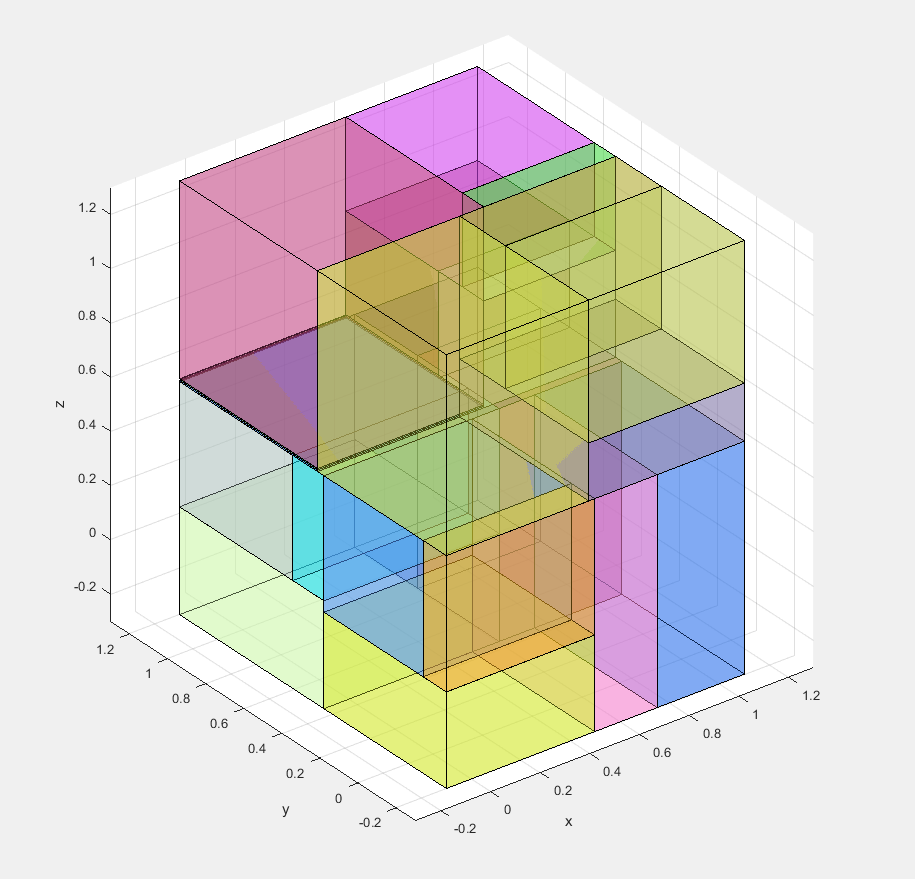
\includegraphics[width=0.65\textwidth]{images/squares.png}
		\vspace{-15pt}
		\caption{Example of $k$-d tree partitions}
	\end{figure}
	
\end{frame}


\subsection{Other tests}

\begin{frame}	
	\frametitle{Validation}
	
	\begin{block}{Other validation methods:}
		\begin{itemize}
			\item Set radius very large, find all points
			\item Set search sphere center on a data point, use tiny radius, find 1 point
			\item Set an arbitrary search sphere point, increase radius, points found increases monotonically
			\item Vary number of compute nodes (altering tree structure), find consistent number of points
			\item \texttt{dumpTree} writes each compute node's tree to a file for analysis
		\end{itemize}
	\end{block}
	
\end{frame}




%%%%%%%%%%%%%
%%%
%%% Section: Results
%%%
%%%%%%%%%%%%%
\section{Results}

\begin{frame}	
	\begin{Huge}
		\begin{center}
			Results
		\end{center}
	\end{Huge}
\end{frame}

%%%
% By function analysis
%%%

\begin{frame}[fragile]	
	\frametitle{Timing Data}
	
        	\begin{block}{By function}
        		\begin{itemize}
        			\item Test data was 5,000,000 total data rows and 1,000 search rows on 4 cores
        			\item I/O was the primary bottleneck: disk for \texttt{importFiles} and network for \texttt{buildTree}
        		\end{itemize}
        	\end{block}
        	\begin{figure}
            \centering
	        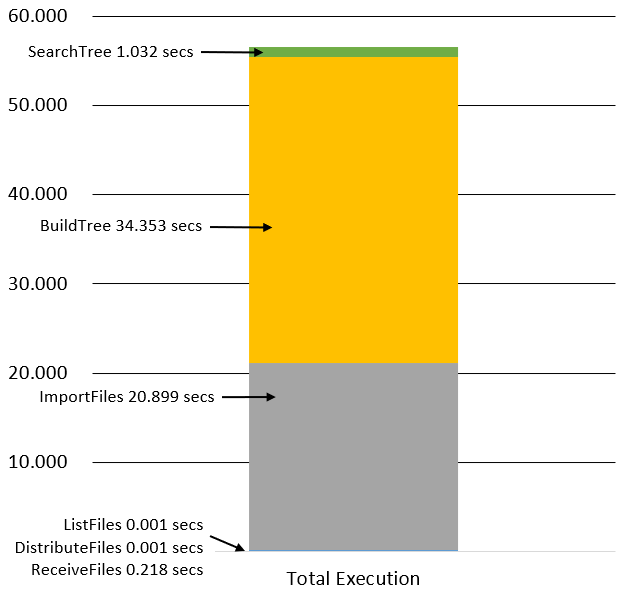
\includegraphics[width=0.40\textwidth]{images/Runtime3.png}
	        \end{figure}
\end{frame}


%%%
% Few total lines
%%%

\begin{frame}[fragile]	
	\frametitle{Timing Data}
	
        	\begin{block}{Performance}
        		\begin{itemize}
        			\item For fewer that 45,000,000 data rows 128 nodes performed best
        		\end{itemize}
        	\end{block}
        	\begin{figure}
            \centering
	        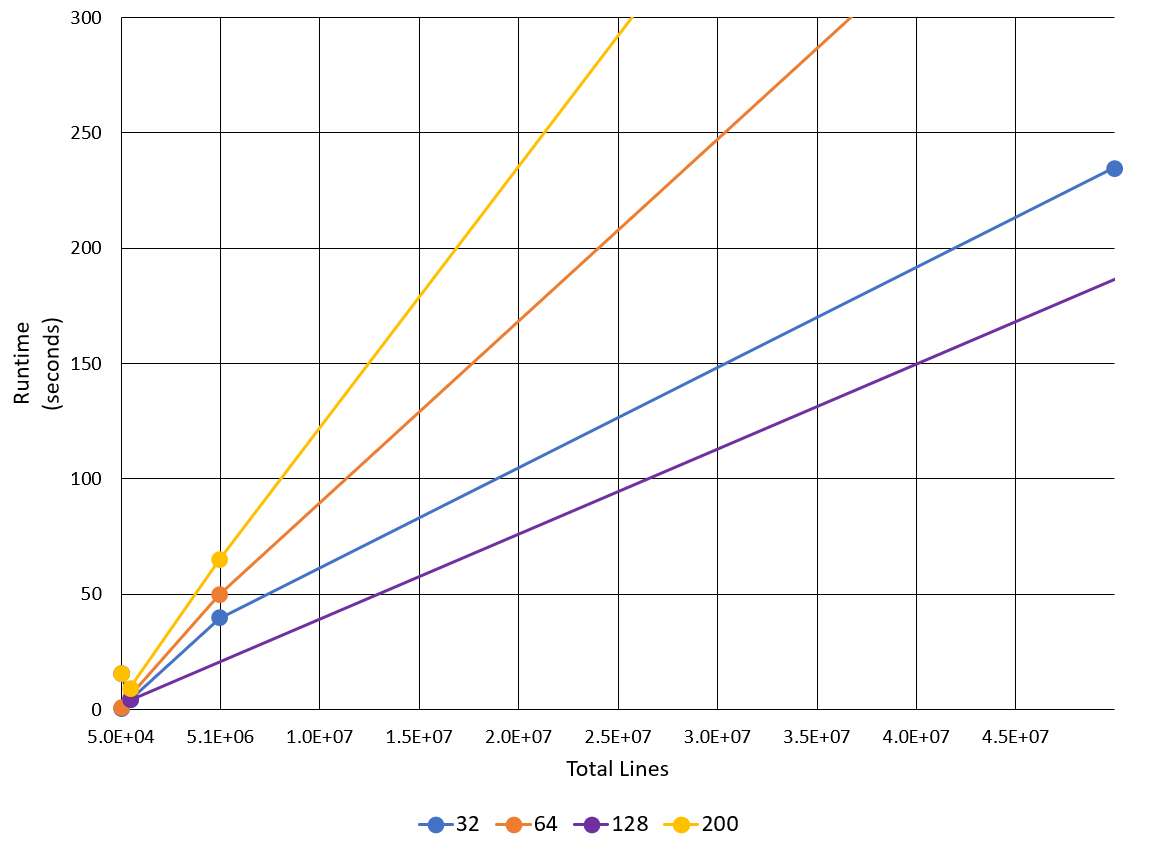
\includegraphics[width=0.7\textwidth]{images/Runtime1.png}
	        \end{figure}
\end{frame}

%%%
% More lines
%%%

\begin{frame}[fragile]	
	\frametitle{Timing Data}
	
        	\begin{block}{Performance}
        		\begin{itemize}
        			\item Overall, 32 cores performed equivalently to 128 cores
        			\item 200 cores was the worst performer
        		\end{itemize}
        	\end{block}
        	\begin{figure}
            \centering
	        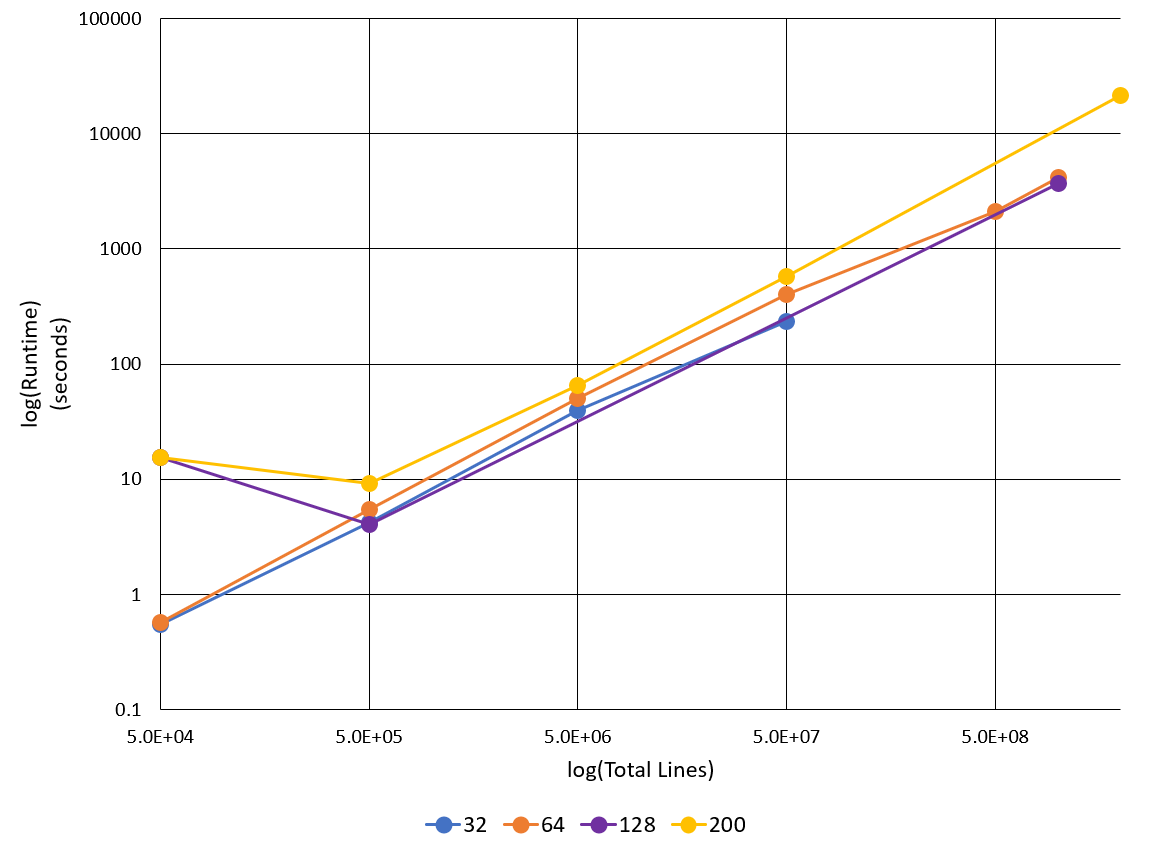
\includegraphics[width=0.65\textwidth]{images/Runtime2.png}
	        \end{figure}
\end{frame}

%%%
% Everything
%%%

\begin{frame}[fragile]	
	\frametitle{Timing Data}
	
        	\begin{block}{Scalability}
        		\begin{itemize}
        			\item Overall, 32 cores performed equivalently to 128 cores
        			\item 200 cores was the worst performer
        		\end{itemize}
        	\end{block}
        	\begin{figure}
            \centering
	        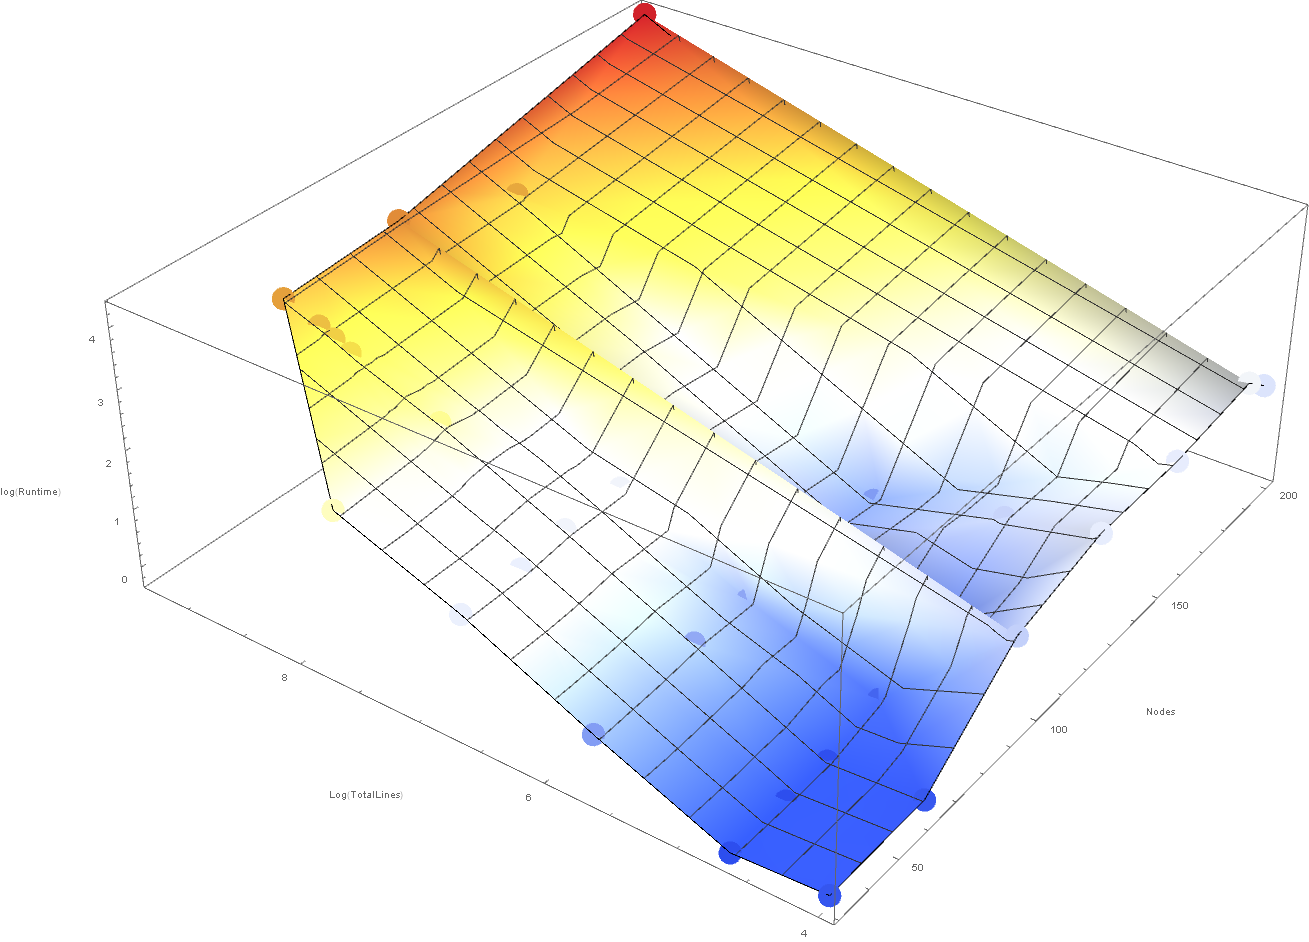
\includegraphics[width=0.65\textwidth]{images/runtimes.png}
	        \end{figure}
\end{frame}

%%%
% Search
%%%

\begin{frame}[fragile]	
	\frametitle{Search Results}
	
        	\begin{block}{Output}
\begin{verbatim}
POINTS FOUND:
   X          Y          Z        0.01      0.05      0.10
--------  ---------  ---------  -------  --------  --------
0.581959   0.721012   0.969341   917205  55498018  92120227
0.894312   0.362959   0.447526    13375   1634169  12135389
0.801765  -0.037433   0.616920     4026    490535   3837163
0.685972   0.346683   0.388596    29251   3420777  22785611
0.716828   0.953059   0.275552     3771    462728   3675457
0.113410   0.650905   0.795308   797814  53199022  78642100
0.125404   0.282296   0.536048     1473    187628   1556214
0.557424   0.471667  -0.075745     1559    190467   1523646
0.557737   0.697675   0.934643   819217  52896281  92109359
0.353073   0.840097  -0.000039     1631    195440   1564030
0.365097   0.064303   0.803032    13811   1693414  12855261
\end{verbatim}
        	\end{block}
\end{frame}


%%%%%%%%%%%%%
%%% NEW SECTION %%%
%%%%%%%%%%%%%
\section{Conclusions}

\begin{frame}	
	\begin{Huge}
		\begin{center}
			Conclusions
		\end{center}
	\end{Huge}
\end{frame}

\subsection{Challenges}

\begin{frame}	
	\frametitle{Challenges}
	
	\begin{alertblock}{Challenges:}
		\begin{itemize}
		\item memory management (leaks, limited space, Signal 9)
		\item array out of bounds issues
		\item multiple communicators (comm)
		\item no planning for function arguments and return values (constant editing of h-files)
		\item testing was difficult due to cluster overloading and hardware errors
		\item debug print statement clutter
		\item inconsistent usage pointer-to-pointer calls for *data[] and *rows (due to \texttt{swapArrayParts})
		\item \texttt{malloc} when you should \texttt{realloc}
		\item \texttt{parallelSort} conversions
		\item \texttt{adaptBins} convergence problems
		\end{itemize}
	\end{alertblock}

\end{frame}

\begin{frame}	
	\frametitle{Challenges}
	
	\begin{alertblock}{\small Annoying personality quirks and idiotic coding habits:}
		% so put your complaints about each other here LOL (all that sand tho)
		\begin{itemize}
			\small
			\setlength\itemsep{0.1pt}
			\item Graham: \\ \vspace{-5pt}
				\begin{itemize}
					\small
					\setlength\itemsep{0.1pt}
					\item Obsessive fixation on the most minor of convention details (can't see the forest for the trees)
					\item So many windows open! How do you find anything?
					\item Always has to try it the wrong way before doing what James suggested 10 minutes earlier \vspace{-5pt}
				\end{itemize}
			\item James: \\ \vspace{-5pt}
				\begin{itemize}
					\small
					\setlength\itemsep{0.1pt}
					\item Who needs whitespace?
					\item Pointers! Pointers everywhere!
					\item Memory leak? Just run it on more nodes! \vspace{-5pt}
				\end{itemize}
			\item JJ: \\ \vspace{-5pt}
				\begin{itemize}
					\small
					\setlength\itemsep{0.1pt}
					\item Insistent usage of Visual Studio replaces neatly arranged tabs with ugly, inconsistent spaces
					\item SO MUCH debug/timing \texttt{cout} clutter
					\item Naming conventions? Who needs those? (What's a camel case?)
				\end{itemize}
		\end{itemize}
	\end{alertblock}

\end{frame}

\subsection{Successes}

\begin{frame}	
	\frametitle{Successes}
	
	\begin{exampleblock}{Successes:}
		\begin{itemize}
		\item few merge conflicts and fast coding through extreme coding and Git branches
		\item efficient delegation of tasks
		\item visualizing output through MATLAB
		\item excellent validation techniques
		\end{itemize}
	\end{exampleblock}

\end{frame}

\begin{frame}	
	\frametitle{Successes}
	
	\begin{exampleblock}{Helpful personality quirks and proper coding habits:}
		% so put your complaints about each other here LOL (all that sand tho)
		\begin{itemize}
			\setlength\itemsep{0.5pt}
			\item Graham: \\
				\begin{itemize}
					\setlength\itemsep{0.5pt}
					\item I can do math
					\item Obsessive attention to detail pays off when writing the paper/presentation
				\end{itemize}
			\item James: \\
				\begin{itemize}
					\setlength\itemsep{0.5pt}
					\item Engineering mindset provides more efficient solutions to problems
				\end{itemize}
			\item JJ: \\
				\begin{itemize}
					\setlength\itemsep{0.5pt}
					\item C++/Git guru
				\end{itemize}
		\end{itemize}
	\end{exampleblock}

\end{frame}

\subsection{Future Work}

\begin{frame}	
	\frametitle{Future Work}
	
	\begin{block}{Future work:}
		\begin{itemize}
			\item cloud computing
			\item use of coding techniques for personal research
		\end{itemize}
	\end{block}
	
\end{frame}




 
\end{document}
